
\begin{frame}{\lantern - Data \& Models}

    \vspace{-3mm}
    \begin{block}{}
        \begin{columns}[onlytextwidth]
            \column{0.48\textwidth}
            \centering
            \textbf{Input:} features

            \column{0.02\textwidth}

            \column{0.48\textwidth}
            \centering
            \textbf{Output:} target
        \end{columns}

        \pause
        \begin{columns}[onlytextwidth]
            \column{0.48\textwidth}
            \centering
            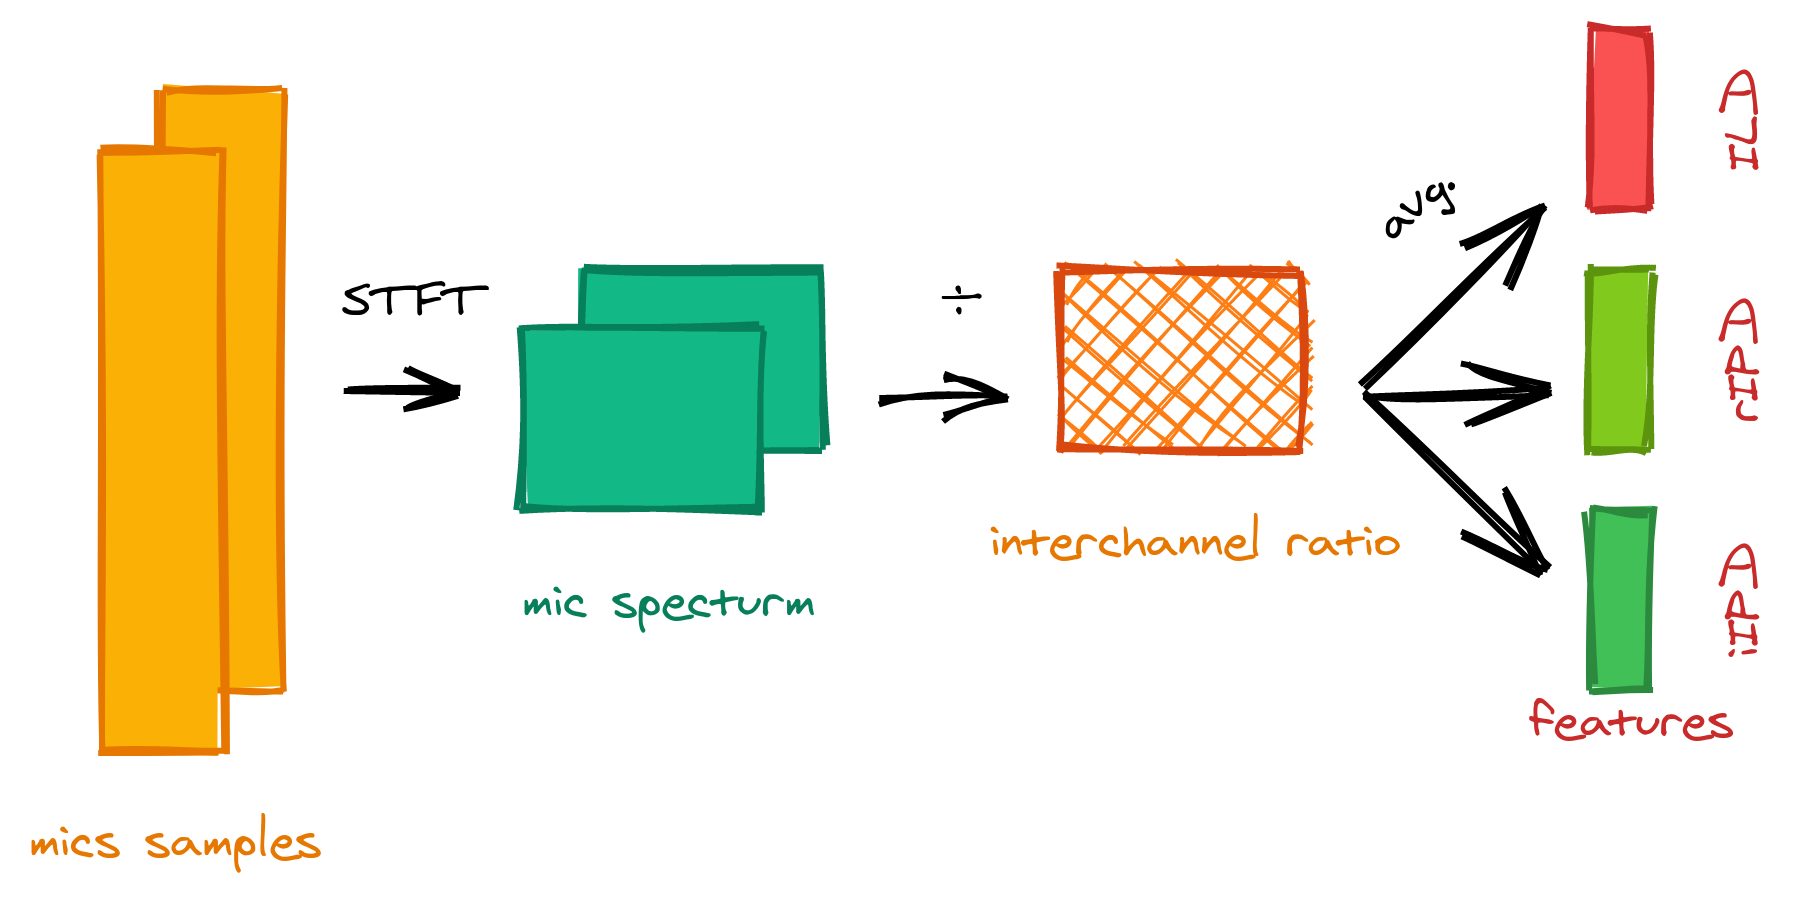
\includegraphics[width=\textwidth]{figures/lantern.png}

            \column{0.02\textwidth}
            $\longrightarrow$

            \column{0.48\textwidth}
            \centering
            % \only<2>{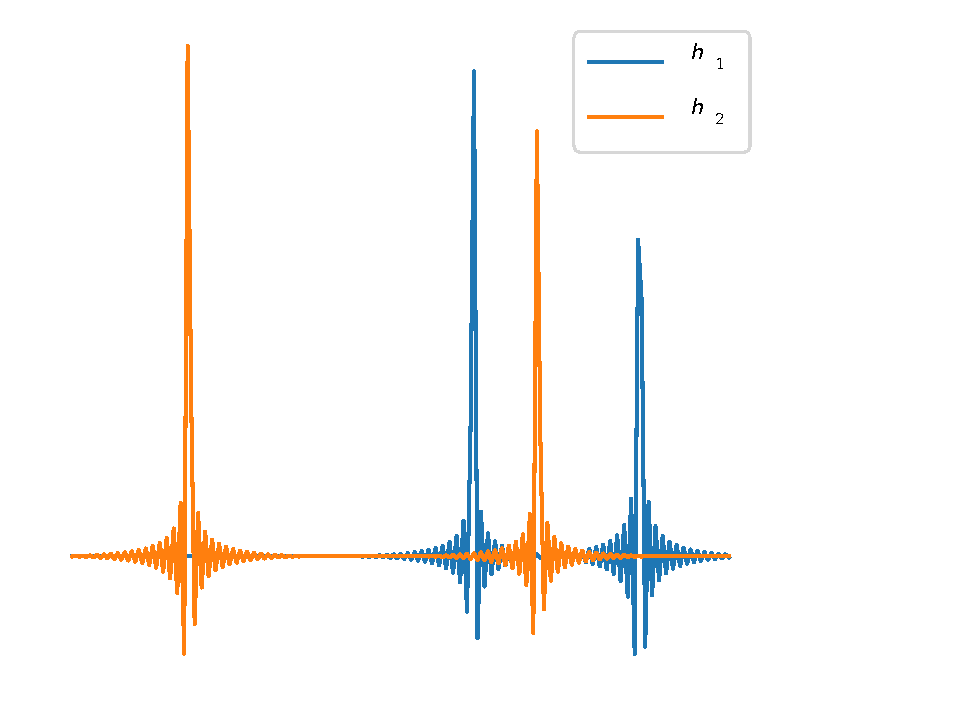
\includegraphics[width=40mm]{figures/rirs1.pdf}}%
            % \only<3>{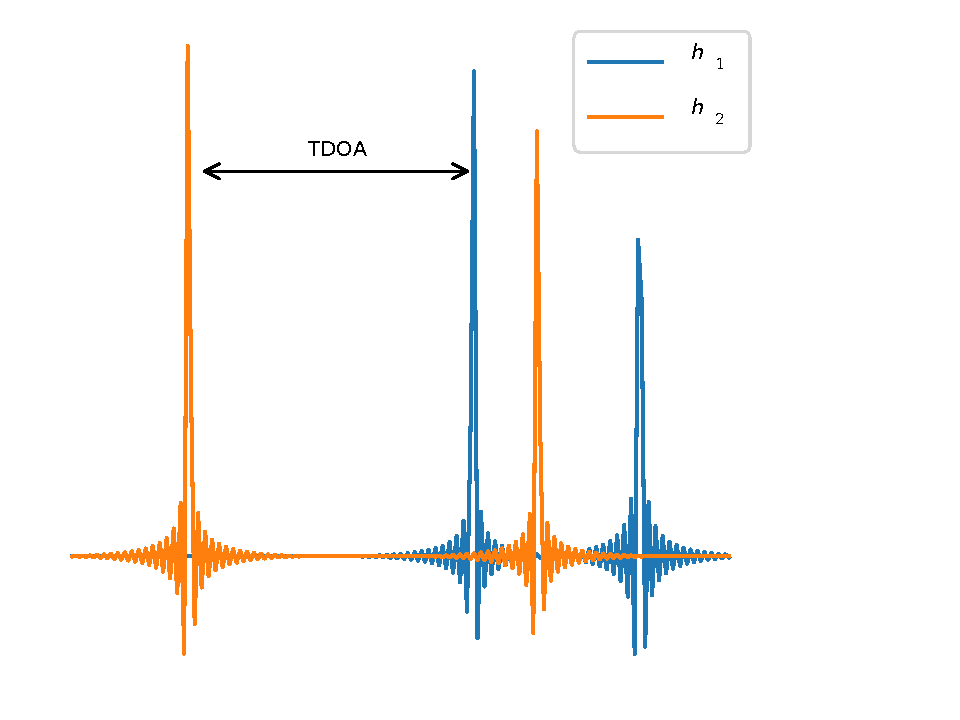
\includegraphics[width=40mm]{figures/rirs2.pdf}}%
            % \only<4>{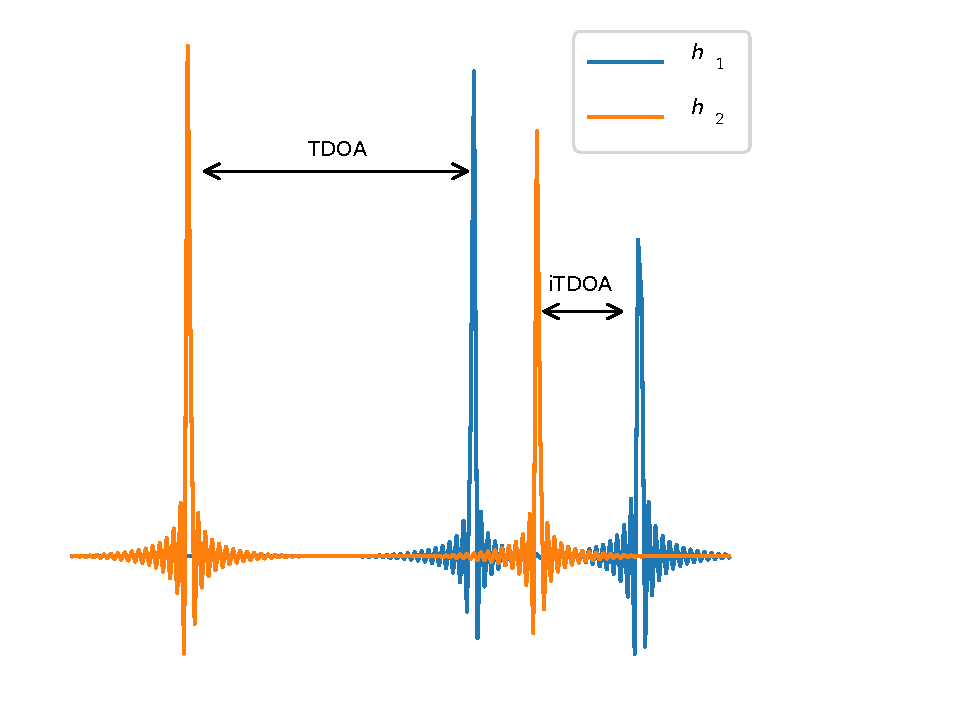
\includegraphics[width=40mm]{figures/rirs3.pdf}}%
            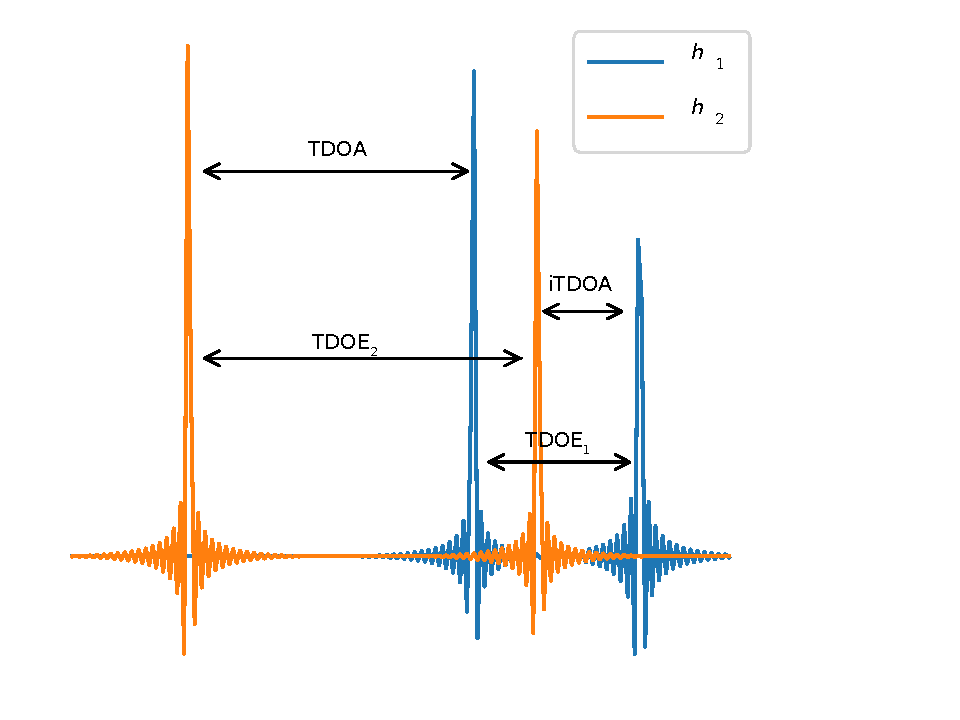
\includegraphics[width=40mm]{figures/rirs4.pdf}
        \end{columns}

        \begin{columns}[T,onlytextwidth]
            \column{0.48\textwidth}
            \centering
            Relative Transfer Function
            \begin{equation*}
                    \mathtt{ReTF}[f] = \frac{H_2[f]}{H_1[f]} \approx \timeavg \kparen{\frac{X_2[f,t]}{X_1[f,t]}}
            \end{equation*}
            \textcolor{gray}{\small This is the \textbf{instantaneous} $\mathtt{ReTF}$}

            \column{0.02\textwidth}

            \column{0.48\textwidth}
            \centering
            TDOAs inter and intra reflection
            \begin{equation*}
                \mathcal{V} = \kbrace{\mathtt{TDOA}, \mathtt{iTDOA}, \mathtt{TDOE}_1}
        \end{equation*}
        \textcolor{myred}{First strongest echo $\Leftrightarrow$ close surface}
        % \\\textcolor{gray}{\small $\mathtt{TDOE}_2$ is a combination of $\mathcal{V}$}
        \end{columns}
    \end{block}

    \pause
    \begin{block}{Model}
        \begin{itemize}
            \item Architecture: \textbf{CNN}~{\small\cite{chakrabarty2017broadband,nguyen2018autonomous}}

            \pause
            \item Loss Function:
            \begin{enumerate}
                \item RMSE (Multi-label regression) on $\mathcal{V}$
                \item Gaussian log-likelihood $\to \kbrace{\mu, \sigma^2}$\hspace{.8em}\tikzmark{right}\tikzmark{T2}
                \item Student log-likelihood $\to \kbrace{\mu, \lambda, \nu}$\tikzmark{B2}
            \end{enumerate}

            \pause
            \item Virtually Supervised Learning (= data from acoustic simulator)
        \end{itemize}

    \end{block}

    \pause
    \begin{tikzpicture}[overlay, remember picture]
        \node[anchor=base] (a) at (pic cs:T2) {\vphantom{h}}; % push the mark to the top of the line (ie including ascenders)
        \node[anchor=base] (b) at (pic cs:B2) {\vphantom{g}}; % push the mark to the bottom of the line (ie including descenders)
        \draw [decoration={brace,amplitude=0.35em},decorate,thick,gray]
         (a.north -| {pic cs:right}) -- node[right,inner sep=1em] {
             \small Generative models $\gets$ \parbox{12em}{for data fusion
                                                           \\similar to \textbf{MDN}~{\footnotesize\cite{bishop1994mixture}}}
          } (b.south -| {pic cs:right});
    \end{tikzpicture}

\end{frame}


\begin{frame}[t]{\lantern - Experiments \& Resuls}

    \vspace*{-0.5em}
    \begin{columns}[T]
            \begin{column}{0.60\textwidth}

                \begin{description}
                    \item[Baseline:] $\mathtt{GCCPHAT}$ (only TDOA),
                                    \\$\mathtt{MLP}_{\calV}$~\cite{di2019mirage}
                    \item[Proposed:] $\mathtt{CNN}_{\calV}$, $\mathtt{CNN}_{\calV_{\calN}}$, $\mathtt{CNN}_{\calV_{\calT}}$

                    \pause
                    \item[Metric:] normalized RMSE
                                    \\(0 = best fit, 1 = random)
                \end{description}

            \end{column}

            \pause
            \begin{column}{0.35\textwidth}
            \small
            Train:
            \begin{itemize}
                \item random RT60, random SNR
                \item broadband source (wn)
                \item instantaneous RTF
            \end{itemize}
            Test: similar to train

        \end{column}

    \end{columns}

    \pause[3]

    \only<4>{
    \begin{block}{}
        \centering
        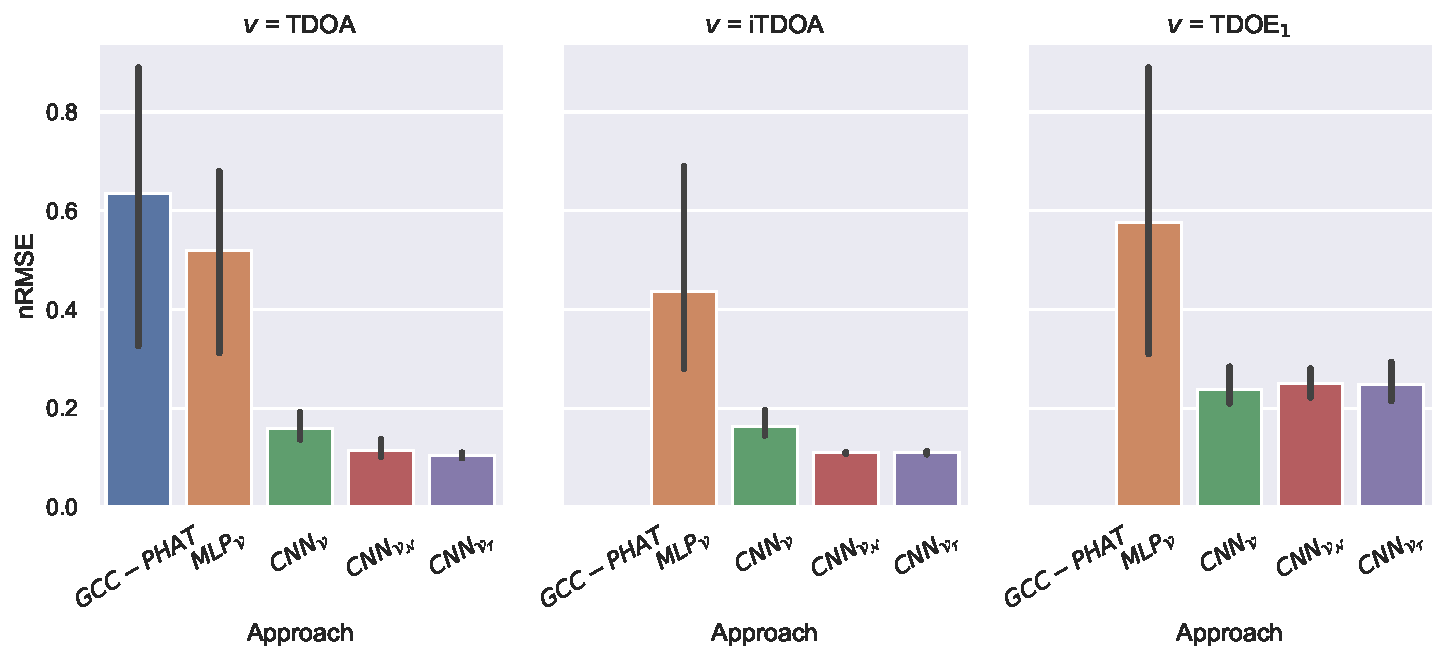
\includegraphics[width=0.9\textwidth]{figures/lantern_snr10.pdf}
    \end{block}

    \begin{center}
        \textcolor{mygreen}{\cmark \: \parbox{8em}{CNNs outperform\\GCC-PHAT, MLP}}
        \quad\textcolor{mygreen}{\cmark \: \parbox{8em}{CNNs\\less variance}} % see the variance
        \quad\textcolor{myred}{\xmark \: \parbox{8em}{Gaussian\\$\sim$ Student-T}}
    \end{center}
    }

    \only<5>{
    \begin{block}{}
        \centering
        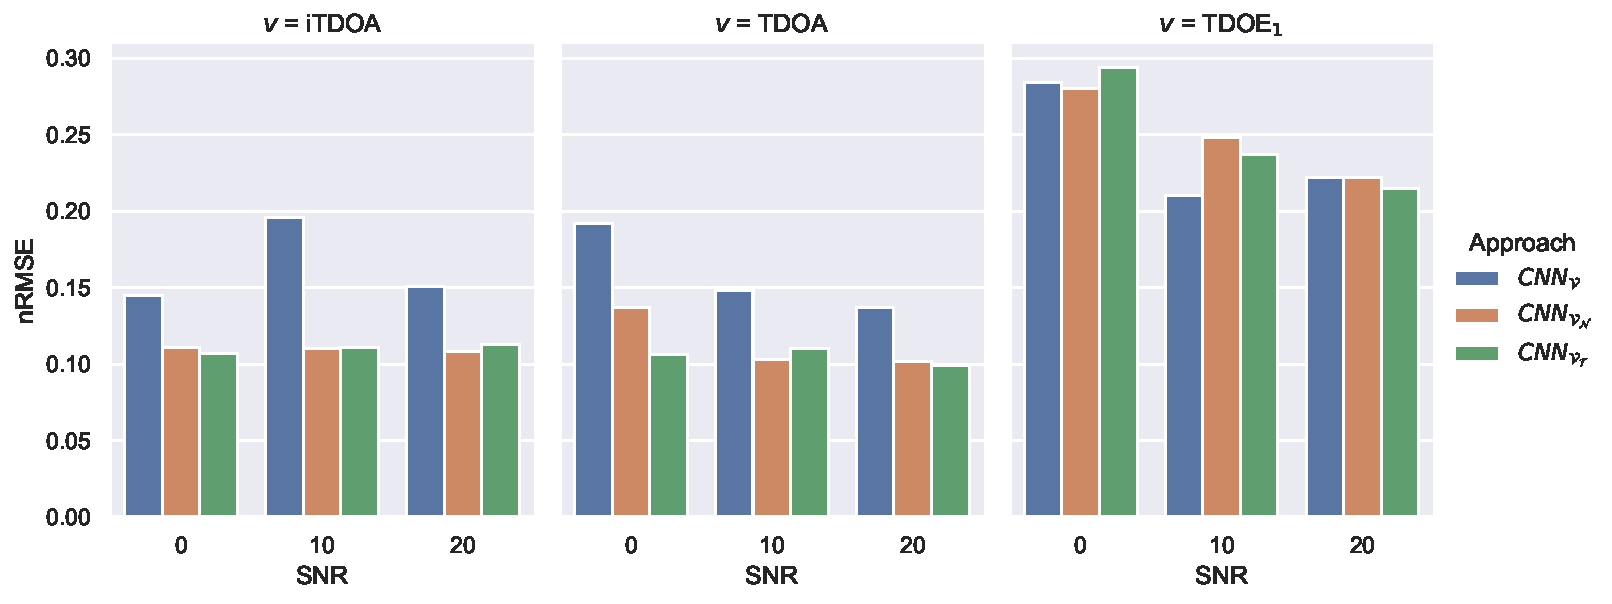
\includegraphics[width=0.9\textwidth]{figures/lantern_snr.pdf}
    \end{block}

    \begin{center}
        \textcolor{mygreen}{\cmark \: \parbox{8em}{Generative\\better than\\Normal}}
        \quad\textcolor{myred}{\xmark \: \parbox{8em}{Gaussian\\$\sim$ Student-T}}
        \quad\textcolor{myred}{\xmark \: \parbox{8em}{Bigger error on TDOE}}
    \end{center}
    }

\end{frame}